\chapter{Troubleshooting}
\label{sec:troubleshooting}

\section{Known Issues}

All known issues in this section concern the Linux AppImage. \\

\subsection{CentOS Fuse Usermount Permissions}

On some operating systems, the following error message is shown when starting the AppImage:

\begin{verbatim}
fuse: failed to exec fusermount: Permission denied

Cannot mount AppImage, please check your FUSE setup.
You might still be able to extract the contents of this AppImage 
if you run it with the --appimage-extract option. 
See https://github.com/AppImage/AppImageKit/wiki/FUSE 
for more information
open dir error: No such file or directory
\end{verbatim}


As the message states, the current user has no permissions to correctly mount the AppImage. Please refer to the provided link \url{https://github.com/AppImage/AppImageKit/wiki/FUSE} for information how to resolve this.

\subsection{Missing glibc Library Versions}

On some operating systems, the following error message is shown when starting the AppImage:\\\\

\begin{verbatim}
/lib64/libc.so.6: version `GLIBC_2.14' not found (required by ...)
/usr/lib64/libstdc++.so.6: version `GLIBCXX_3.4.14' not found (required by ...)
/usr/lib64/libstdc++.so.6: version `GLIBCXX_3.4.15' not found (required by ...)
/lib64/libc.so.6: version `GLIBC_2.14' not found 
  (required by /tmp/.mount_COMPASS-XWB8RF/appdir/bin/../lib/libosgDB.so.130)
...
\end{verbatim}

As stated in \url{https://github.com/AppImage/AppImageKit/issues/398}: \\

``...inside the AppImage requires a newer glibc version than is present on your target system (CentOS 6.7 in your example). The recommended way to produce an AppImage that would run on CentOS 6.7 would be to build on CentOS 6.x...''\\\\

Unfortunately this means that for e.g. CentOS 6.* (or older) an AppImage produced using Ubuntu 14.04 will not run, and currently there no plans to build one (unless requested by large number of users).\\

If this is the case for you please comment on \url{https://github.com/hpuhr/COMPASS/issues/35}.


\subsection{White Geographic View \& Shader Errors in Console Log}
\label{ref:issue_shaders}

When the Geographic View is started on older, unsupported Intel graphics cards the Geographic View only show a white window and the following error messages are logged in the console:

\begin{lstlisting}
...
glLinkProgram 0x1af6a320"" FAILED

VERTEX glCompileShader "main(vertex)" FAILED
VERTEX Shader "main(vertex)" infolog:
0:1(10): error: GLSL 3.30 is not supported. Supported versions are: 1.10, 1.20, 1.30, 1.00 ES, 3.00 ES, and 3.10 ES

FRAGMENT glCompileShader "main(fragment)" FAILED
FRAGMENT Shader "main(fragment)" infolog:
0:1(10): error: GLSL 3.30 is not supported. Supported versions are: 1.10, 1.20, 1.30, 1.00 ES, 3.00 ES, and 3.10 ES

Program "" infolog:
error: linking with uncompiled/unspecialized shadererror: linking with uncompiled/unspecialized shadererror: linking with uncompiled/unspecialized shadererror: linking with uncompiled/unspecialized shadererror: linking with uncompiled/unspecialized shadererror: linking with uncompiled/unspecialized shadererror: linking with uncompiled/unspecialized shadererror: linking with uncompiled/unspecialized shadererror: linking with uncompiled/unspecialized shadererror: linking with uncompiled/unspecialized shadererror: linking with uncompiled/unspecialized shadererror: linking with uncompiled/unspecialized shader
glLinkProgram 0x82eefa0"" FAILED
\end{lstlisting}
\ \\

This is due to the the used graphics libraries OpenSceneGraph and osgEarth depending on shaders defined in GLSL 3.30 (shading language version) and the used graphics card driver not supporting this version of shaders. \\

There exists a workaround which might work for you: There exists the issue that in some cases the shaders are supported in the used Mesa graphics driver, but are not detected correctly. One can override the reported OpenGL version for one application using a system variable and start the app in that mode using:

\begin{lstlisting}
MESA_GL_VERSION_OVERRIDE=3.3 ./COMPASS_1.1.0-x86_64.AppImage
\end{lstlisting}

At least on the authors workstation with an Intel graphics card and for some other users this resolved the issue. \\

If this is not the case for you please comment on \url{https://github.com/hpuhr/COMPASS/issues/151}

\subsection{OpenStreetMap Display Wrong}

When the Geographic View is in an operating system with a Mesa 23 version, the following display issue occurs.

\begin{figure}[H]
    \centering
    \hspace*{-2cm}
    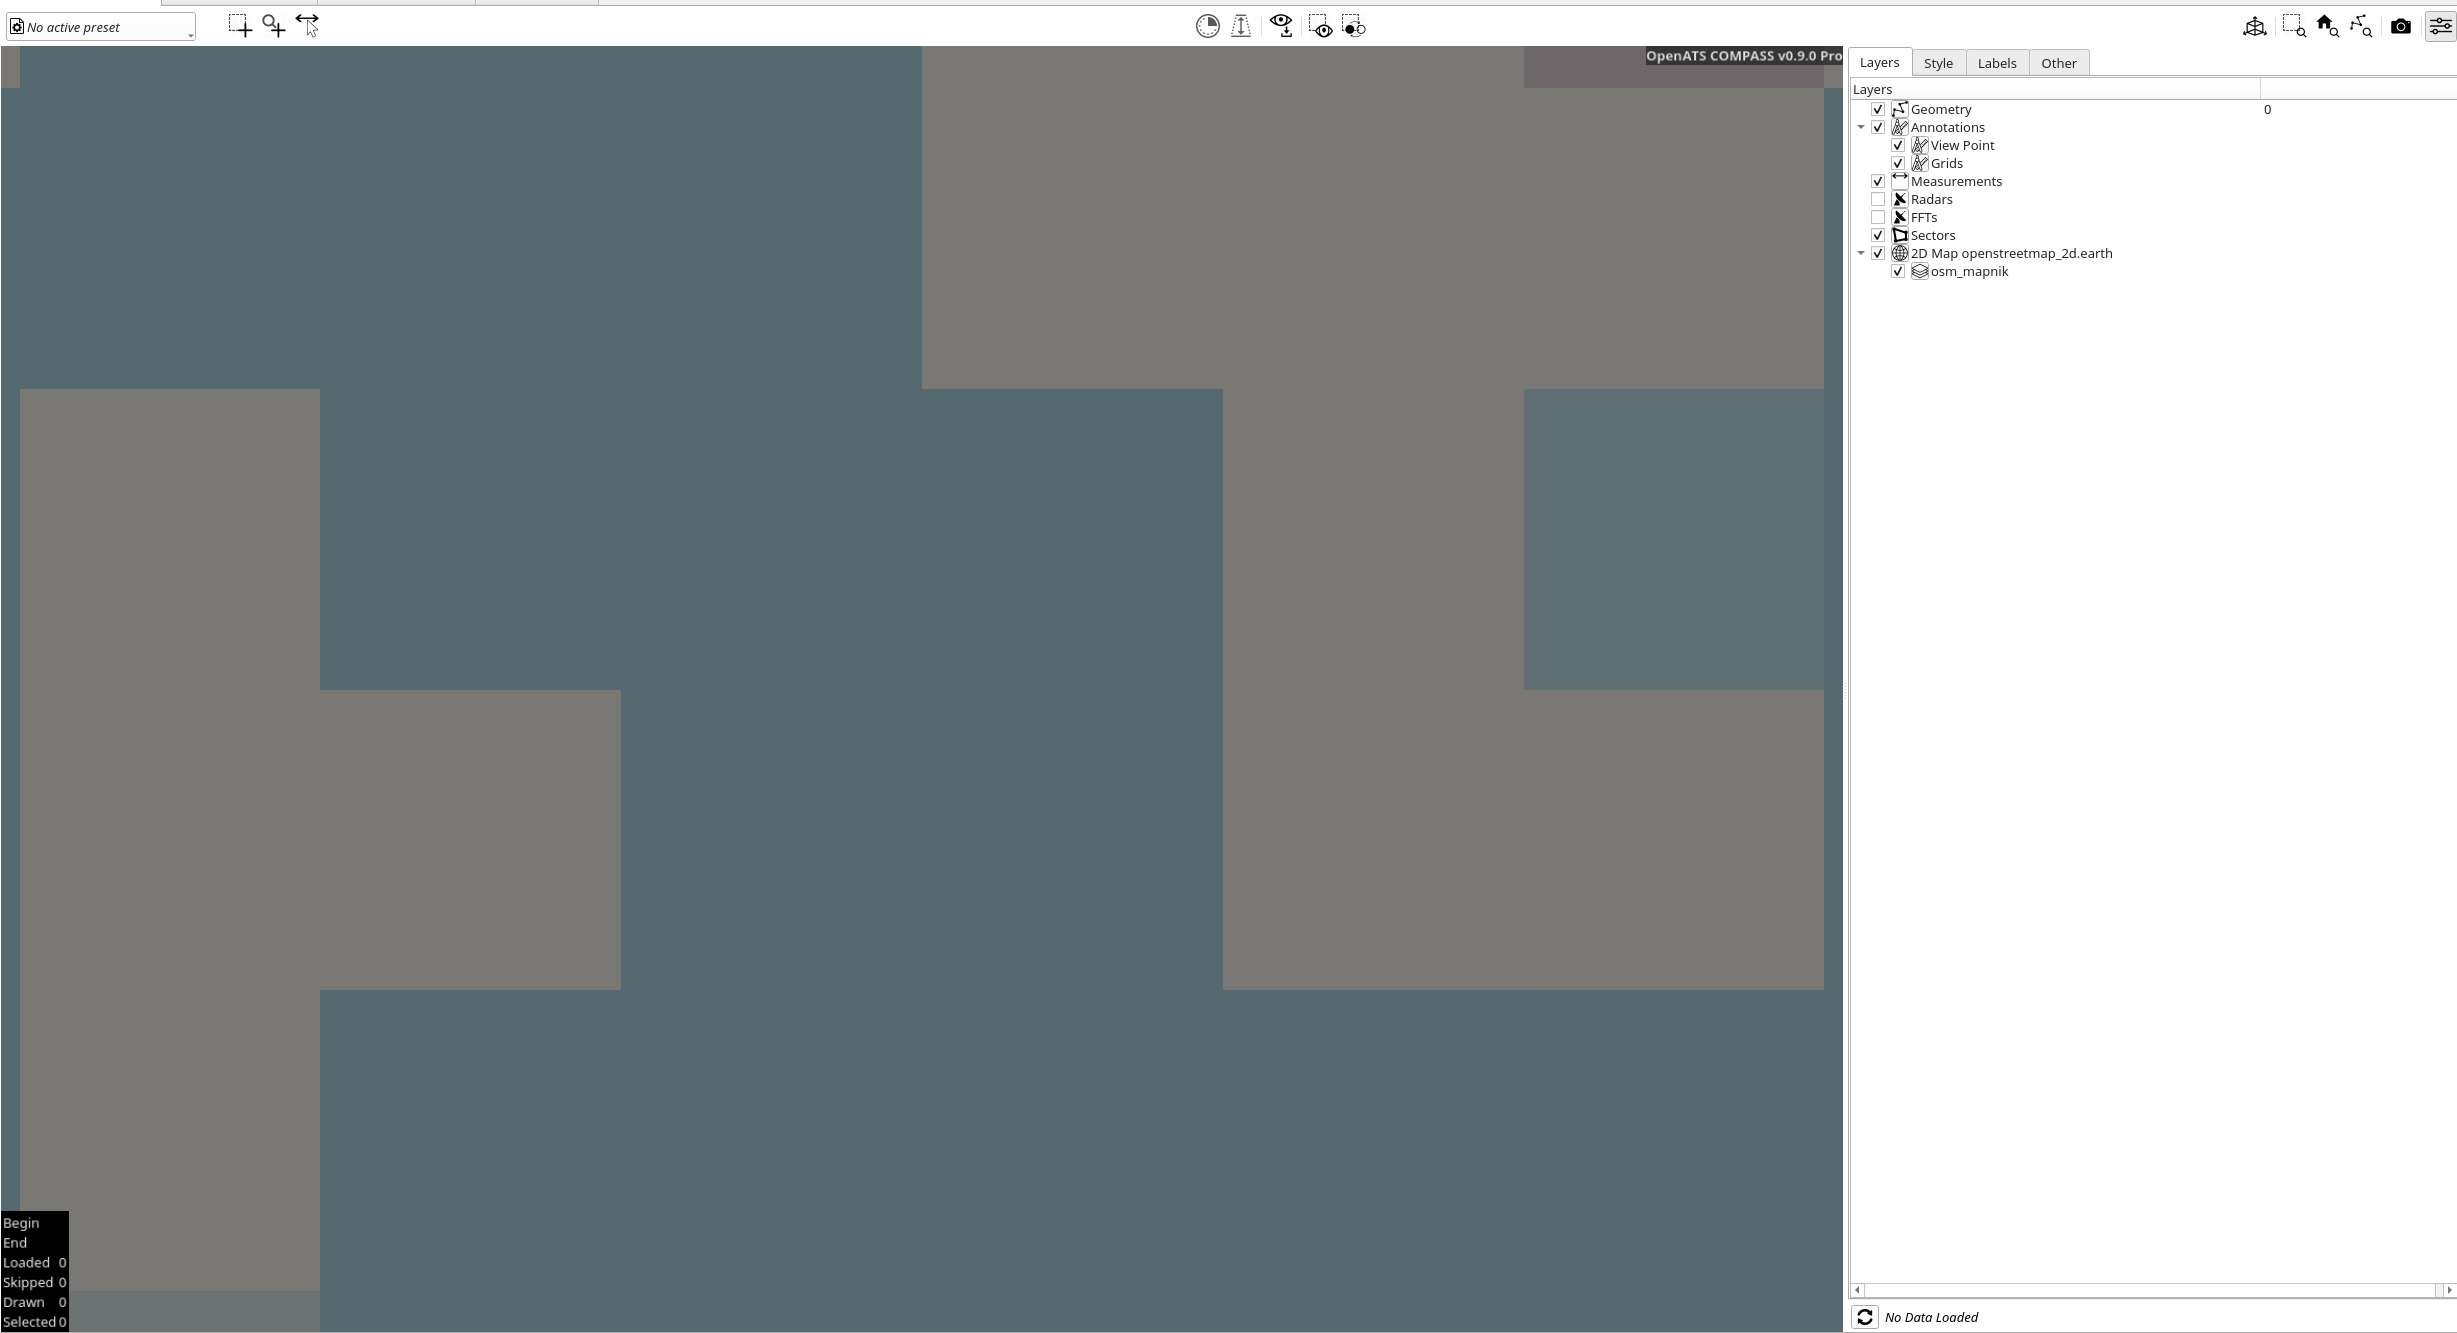
\includegraphics[width=18cm,frame]{figures/geo_osm.png}
  \caption{Geographic View OpenStreetMap Issue}
\end{figure}

The root cause is a known bug in one of the used libraries, the Mesa library. The Mesa API acts as the middleman: Applications call OpenGL functions, Mesa's libGL dispatches to the appropriate DRI driver, which Hardware-specific driver executes on GPU. This Mesa library, in exactly version 23 (and sub-versions) exhibits this issue. \\

Unfortunately, this can not be solved in the application, and no known workarounds exist. The only known solutions are:
\begin{itemize}  
\item Using a different background map (e.g. minimal\_2d)
\item Downgrading to Mesa 22.*
\item Upgrading to Mesa 24.* or later
\end{itemize}
\ \\

It might be possible to resolve this inside COMPASS at a later release, but nothing can be promised for now.

\subsection{Graphical Issues}

For issues of the following nature:

\begin{itemize} 
\item Application might not even start (OpenGl version error)
\item Slow display performance
\item Graphical display errors (wrong colors, artifacts, etc)
\end{itemize} 

If such a display issue exists, additional information is required. \\

Please \textbf{verify} that the installed graphics card and driver in use match the supported version stated in \nameref{sec:graphics_installation}. \\

Only if this is the case, please collect the output of \textit{glxinfo} and create an issue report as stated below. \\

If the application should immediately crash on startup giving an error similar to

\begin{verbatim}
GLib-GIO-ERROR **: 10:47:18.464: Settings schema 'org.gnome.settings-daemon.
plugins.xsettings' does not contain a key named 'antialiasing'
\end{verbatim}

a possible fix can be to start the application using 

\begin{verbatim}
GDK_BACKEND=X11 ./COMPASS_1.1.0-x86_64.AppImage
\end{verbatim}

\section{Reporting Issues}

There are several ways of reporting issues. The following steps have to be taken:

\begin{itemize}  
\item Check if the issue was already reported
\item Collect all required information
\item Report the issue
\end{itemize} 

Please also make sure that you are using the latest version of COMPASS, since the issue might already have been corrected in the current version. \\

Also, if you're planning on using COMPASS, it is of benefit if you register on \url{https://github.com}, which can be done for free. It is then possible for you to comment on issues, create new ones or even contribute to the project.

\subsection{Already Reported Issues}

Please refer to \url{https://github.com/hpuhr/COMPASS/issues} for a list of the currently known issues. An issue can be ``Open'' meaning it was not yet fixed, or ``Closed'', meaning it was at least fixed in the source code. If it is closed, it does not mean that the fix is already included in the current release, but that it will be in the next release. \\

Please look through the issues and make sure that yours isn't already listed. If so, you can comment on it to indicate the severity for you. If not, please proceed to the next step.

\subsection{Collect Information}

Basically everything that is needed to reproduce the error should be submitted. Depending on the type of the error, this can differ, but at least the following information should be given:

\begin{itemize}  
\item Log file of the session with the error, see \nameref{sec:issues_log_files}
\item Exact steps taken until the error occured
\end{itemize} 

\subsubsection{Log Files}
\label{sec:issues_log_files}

COMPASS writes a log file for each start of the application:

\begin{itemize}
\item Folder: the subfolder \texttt{log} of the configuration folder (see \nameref{sec:install_config_folder}):
\begin{itemize}
\item Linux: \texttt{\textasciitilde/.compass/<version>/log/}, e.g. \texttt{/home/<user>/.compass/1.1.0/log/}
\item Windows: \texttt{C:\textbackslash Users\textbackslash <user>\textbackslash .compass\textbackslash <version>\textbackslash log\textbackslash}
\end{itemize}
\item File name: \texttt{compass\_<date>\_<time>\_<process id>.log}, with the date and time of the start, e.g. \texttt{compass\_2026-11-23\_20-59-53\_21396.log}
\item Contents:
\begin{itemize}
\item The same messages as the console, each with date and time
\item After a crash: a crash report at the end of the file, with the stack trace (function, source file and line of each step)
\end{itemize}
\item Size:
\begin{itemize}
\item At most 5 MB per file
\item A full file is renamed to \texttt{.log.1} and a new file is started, so the file pair holds the last 5 to 10 MB of the session
\end{itemize}
\item Only the log files of the last 10 starts are kept, older files are deleted at the start of COMPASS
\end{itemize}
\ \\

The console shows the path of the log file at the start of COMPASS, in a line like this (shortened):
\begin{verbatim}
COMPASSClient: initializing logger using '...', log file
'~/.compass/1.1.0/log/compass_2026-11-23_20-59-53_21396.log'
\end{verbatim}

To report an issue:
\begin{itemize}
\item Find the log file of the session with the error, by the start time in the file name
\item Attach the log file to the report, and the \texttt{.log.1} file of the session if it exists
\end{itemize}
\ \\


\includegraphics[width=0.5cm]{../../data/icons/hint.png} Please \textbf{note} that the log file of a session is deleted after 10 further starts. Copy the log file of the session with the error to another folder before you start COMPASS again several times. \\


\includegraphics[width=0.5cm]{../../data/icons/hint.png} The console log (see \nameref{sec:appendix_logging}) is not changed by the log file, it still shows all messages. \\

\subsubsection{For Application Crashes}
\label{sec:issues_crashes}

If the application crashes, its crash handler writes a crash report:

\begin{itemize}
\item Contents:
\begin{itemize}
\item The type of the error, e.g. an access violation, a signal, a failed internal check or an unhandled error (exception)
\item The stack trace: the function, source file and line of each step that led to the error
\item For an unhandled error: also the stack trace of the place where the error occurred
\end{itemize}
\item Location: at the end of the log file of the session (see \nameref{sec:issues_log_files}) and in the console
\item The console shows the path of the log file after the crash report, in a line \texttt{Log file: <path>}
\end{itemize}
\ \\

The Linux AppImage and \texttt{compass\_handler.exe} on Windows start the application through a watchdog (\texttt{compass\_handler}). The watchdog shows a message:

\begin{itemize}
\item If the application crashes (title \textbf{Application Crash})
\item If the application ends with an error code other than 0, e.g. after a failed internal check (title \textbf{Application Error}). Not with the command line options \texttt{--quit} or \texttt{--open\_rt\_cmd\_port}, so that scripts are not stopped by the message.
\end{itemize}
\ \\

The message shows:

\begin{itemize}
\item The crash or error code of the application
\item The path of the log file with the report
\item \textbf{Open Log File}: Opens the log file with the default text editor
\item \textbf{Open Log Folder}: Opens the folder of the log files
\item \textbf{Close}: Closes the message
\end{itemize}
\ \\

\begin{figure}[H]
    \center
    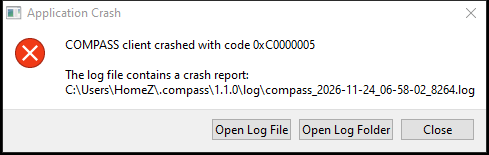
\includegraphics[width=10cm,frame]{figures/crash_message_windows.png}
    \caption{Crash message on Windows}
\end{figure}

\begin{figure}[H]
    \center
    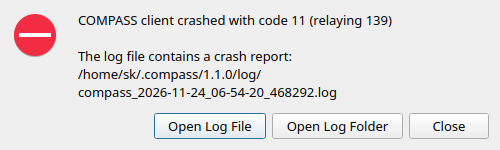
\includegraphics[width=10cm,frame]{figures/crash_message_linux.png}
    \caption{Crash message on Linux}
\end{figure}

To report the crash:

\begin{itemize}
\item Click \textbf{Open Log Folder} and attach the log file shown in the message to the report, and its \texttt{.log.1} file if it exists
\item Describe the steps taken until the crash
\end{itemize}
\ \\


\includegraphics[width=0.5cm]{../../data/icons/hint.png} If \texttt{compass\_client.exe} (Windows) or a self-built \texttt{compass\_client} is started directly, no watchdog runs and no message is shown. The log file and the console still contain the crash report. \\

In some cases a stack trace created manually might be requested. This can be achieved by running the application using gdb (\url{https://www.gnu.org/software/gdb/}), which might have to be installed.

Then, on Linux, the application can be run using \texttt{gdb ./COMPASS\_1.1.0-x86\_64.AppImage}. The output will look similiar to this:

\begin{verbatim}
GNU gdb (Ubuntu 8.0.1-0ubuntu1) 8.0.1
Copyright (C) 2017 Free Software Foundation, Inc.
License GPLv3+: GNU GPL version 3 or later <http://gnu.org/licenses/gpl.html>
This is free software: you are free to change and redistribute it.
There is NO WARRANTY, to the extent permitted by law.  Type "show copying"
and "show warranty" for details.
This GDB was configured as "x86_64-linux-gnu".
Type "show configuration" for configuration details.
For bug reporting instructions, please see:
<http://www.gnu.org/software/gdb/bugs/>.
Find the GDB manual and other documentation resources online at:
<http://www.gnu.org/software/gdb/documentation/>.
For help, type "help".
Type "apropos word" to search for commands related to "word"...
Reading symbols from ./COMPASS-x86_64_RELDBG_0220.AppImage...done.
(gdb) 
\end{verbatim}


In the shown console, enter the command ``run''. This will run the application. Then, perform the same steps as previously to reproduce the application crash.

When the crash occurs, the output should look like this:

\begin{verbatim}
Thread 1 "AppRun" received signal SIGINT, Interrupt.
0x00007fffef950951 in __GI___poll (fds=0x7fffcc007630, nfds=3, timeout=15036) 
at ../sysdeps/unix/sysv/linux/poll.c:29
29	../sysdeps/unix/sysv/linux/poll.c: No such file or directory
\end{verbatim}

Then, enter the command ``backtrace''. This will show output similiar to this:

\begin{verbatim}
#0  0x00007fffef950951 in __GI___poll (fds=0x7fffcc007630, nfds=3, timeout=15036) at 
../sysdeps/unix/sysv/linux/poll.c:29
#1  0x00007fffec5bb169 in ?? () from /lib/x86_64-linux-gnu/libglib-2.0.so.0
#2  0x00007fffec5bb27c in g_main_context_iteration () 
from /lib/x86_64-linux-gnu/libglib-2.0.so.0
#3  0x00007ffff308998c in QEventDispatcherGlib::processEvents
(QFlags<QEventLoop::ProcessEventsFlag>) ()
   from /tmp/.mount_COMPASS-1XB9QP/appdir/bin/../lib/libQt5Core.so.5
#4  0x00007ffff303b96b in QEventLoop::exec(QFlags<QEventLoop::ProcessEventsFlag>)
 () from /tmp/.mount_COMPASS-1XB9QP/appdir/bin/../lib/libQt5Core.so.5
#5  0x00007ffff30420e1 in QCoreApplication::exec() () from 
/tmp/.mount_COMPASS-1XB9QP/appdir/bin/../lib/libQt5Core.so.5
#6  0x00000000006be3c6 in main ()
\end{verbatim}

This is called a stacktrace. Please copy all of this text and add it to the issue report (upon request).


\subsection{Issue Reporting}

Please either create a new issue on GitHub (\url{https://github.com/hpuhr/COMPASS/issues}) or send a mail to \href{mailto:compass@openats.at}{compass@openats.at}, and include all of the previously collected information. \\

If the supplied information is not enough you will be contacted as soon as time allows, with a request for further detail.


